\chapter{Results of the eye tracking experiments}
\label{chap:results}

Here it follows the discussion about the data collected on the participants’ eye movement during the experiments. As explained previously in Section~\ref{sec:fwkdataanalysis}, at the current state of this research is not possible to provide quantitative computations on the eye tracking data. Moreover, the eye tracker experiment software does not provide calculation modules for smooth pursuit eye movements. Complex algorithms need to be applied on the raw data in the future. For these reasons, the analysis is mainly based on the visual inspection of the graphs outputted by the eye tracker software. Therefore, the following analysis is qualitative, subjective and based on the researcher’s interpretation of the framework and of the measurements. Along with the eye tracker recordings, qualitative data were collected for each participant, in the form of written notes, about how they behaved in relation to the whole procedure.

The graphs shown in the following sections show a series of eye parameters, which are enlisted in the legend on the right side of the charts. In particular, the eye position is not shown by the composite cartesian coordinates (x,y), but the two coordinates are plotted separately. Therefore it is not possible to overlap the graphs with the visual stimuli. There are different units of measure on the chart’s axes for the eye positions (pixels), the pupil diameter (mm) and the eye velocity (deg/s). For each participant, a tracking ratio is provided, which reports the percentage of correctly recorded data over the trial total amount.

The eye tracker software also tags the eye movements depending on their features, creating events for fixations, saccades and blinks. However, lacking of the smooth pursuit tag, it is not possible to discern fixations from smooth pursuit eye movements at the moment.

\section{Pilot test [PT]: the reference dataset}
\label{sec:respilot}

Before conducting the experiment, the author conducted a pilot test in order to collect reference data. The data and the eye movement patterns shown in the following charts are the one which are expected to be elicited by the visual stimuli developed for the framework.
The author knows all the stimuli in detail, he does not have any clinical diagnosis, and his eyesight is corrected to normal by glasses. Therefore it can be assumed that his performance on tracking the targets is theoretically one of the best achievable. The tracking ratio for the pilot test is \(\geq\) 95.8\% \begin{comment} (Tab.~\ref{tab:pilotsummary}).

\begin{table}[h]
  \centering
  \begin{tabular}{c|c}
    Age  & IQ  \\ 
    \hline
    10   & 100 \\
    20   & 100 \\
    30   & 150
  \end{tabular}
  \caption{Summary of pilot test trials}
  \label{tab:pilotsummary}
\end{table}
\end{comment}

\subsection{PT\_T1 : Sinusoidal motion visual stimuli}
\label{sec:PT_T1}

\begin{figure}[t]
  \centering
  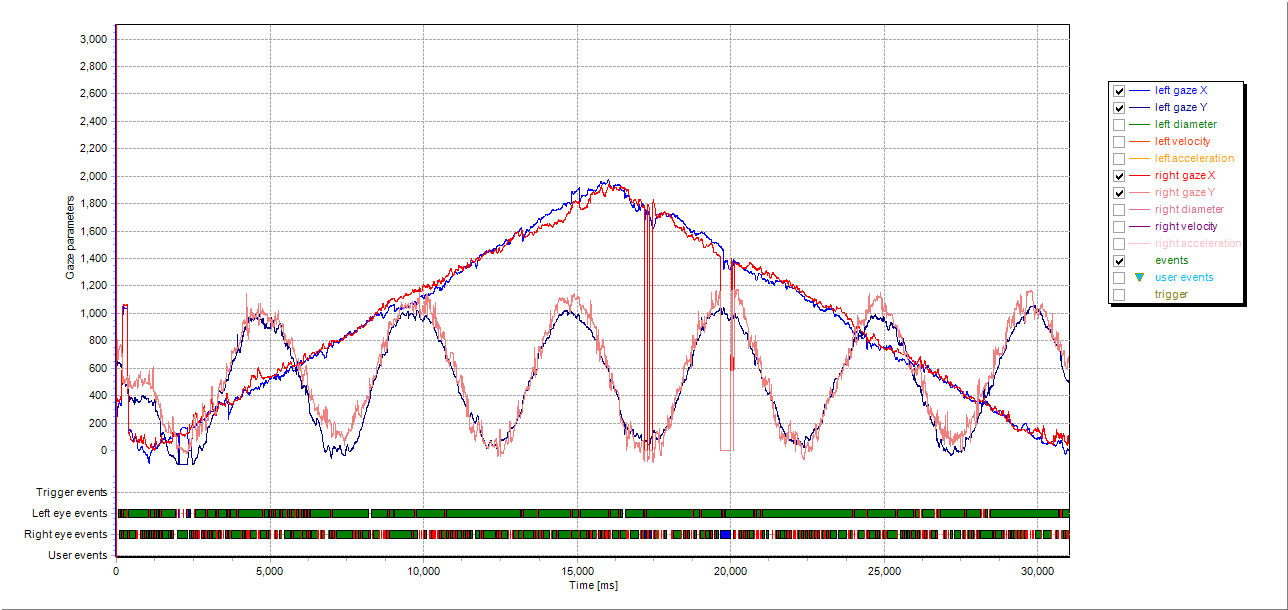
\includegraphics[width=.8\textwidth]{figures/graphs/PT_T1(sinusoid)_XY.png}
  \caption[PT\_T1 Eye positioning]{PT\_T1 Eye positioning}
  \label{fig:PT_T1_pos}
\end{figure}

The sinusoidal tracking pattern (Fig.~\ref{fig:PT_T1_pos}) is evident from the plots of the y coordinate, while from the x coordinate plots it can be inferred that in the first half of the experiment the target moved from left to right (increase of x value) and then it travelled backwards (decrease of x value) following the same pattern (no disruption of the sinusoidal y pattern). The eye movements in the first 1000 ms are due to the focus-to-target routine in the stimuli. From the graph it can be seen that during two changes of directions (17.5 and 20 s) large saccades were performed, probably in the attempt to predict larger movements of the target. The left eye tracks smoothly the target sinusoidal movement with more precision, while the right eye is less precise. This is probably due to the dominance of the left eye over the right one in the subject.

\begin{figure}[t]
  \centering
  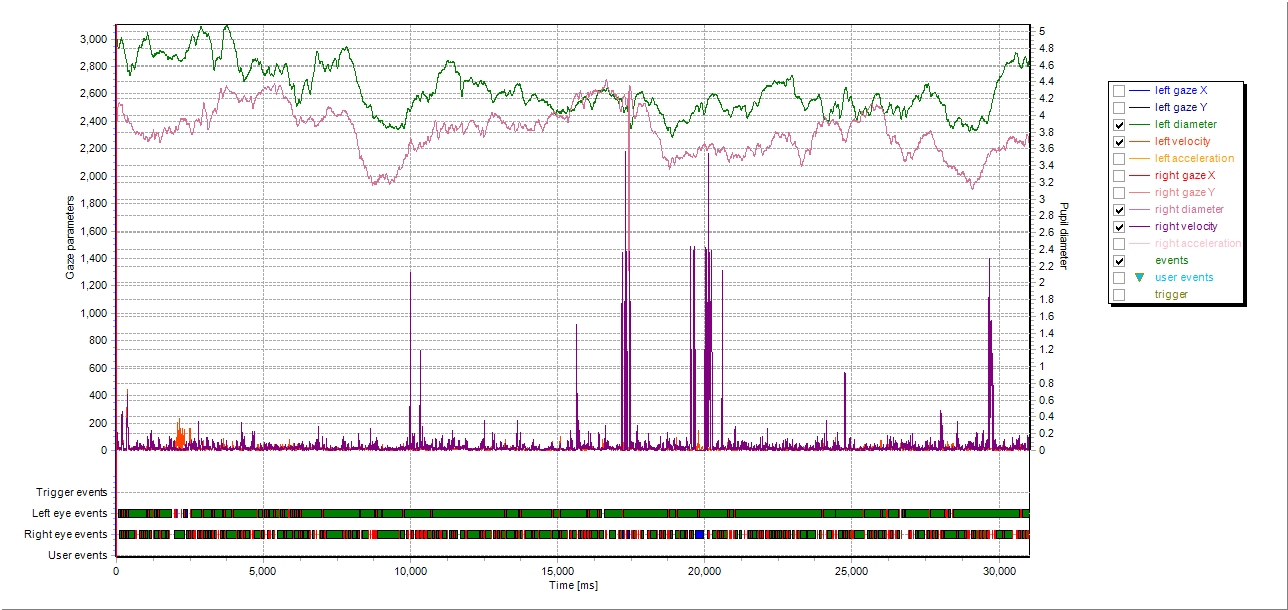
\includegraphics[width=.8\textwidth]{figures/graphs/PT_T1(sinusoid)_VP.png}
  \caption[PT\_T1 Pupil size and velocity profile]{PT\_T1 Pupil diameter and eye velocity}
  \label{fig:PT_T1_vel}
\end{figure}

Fig.~\ref{fig:PT_T1_vel} shows that a number of small saccades (the spikes in the eye velocity profile) were performed during the pursuit, and the two groups of larger saccades discussed in the chart Fig.~\ref{fig:PT_T1_pos} are well highlighted by high peaks of eye velocity.



\subsection{PT\_T2 : Triangular motion visual stimuli}
\label{sec:PT_T2}

\begin{figure}[h]
  \centering
  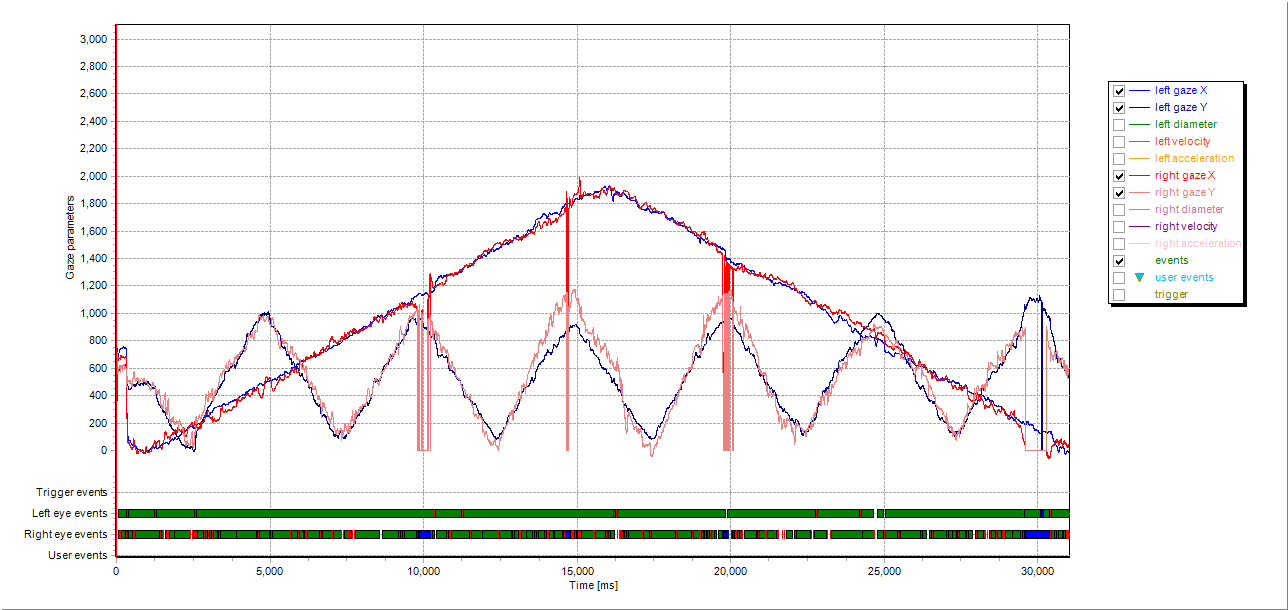
\includegraphics[width=.8\textwidth]{figures/graphs/PT_T2(triangular)_XY.png}
  \caption[PT\_T2 Eye positioning]{PT\_T2 Eye positioning}
  \label{fig:PT_T2_pos}
\end{figure}

The considerations made for the sinusoidal motion chart (Fig.~\ref{fig:PT_T2_pos}) apply here to the triangular motion chart. Here it is even more evident the attempt to perform saccades at turning points of the target motion, which are indeed more abrupt than in the sinusoidal pattern.

\begin{figure}[h]
  \centering
  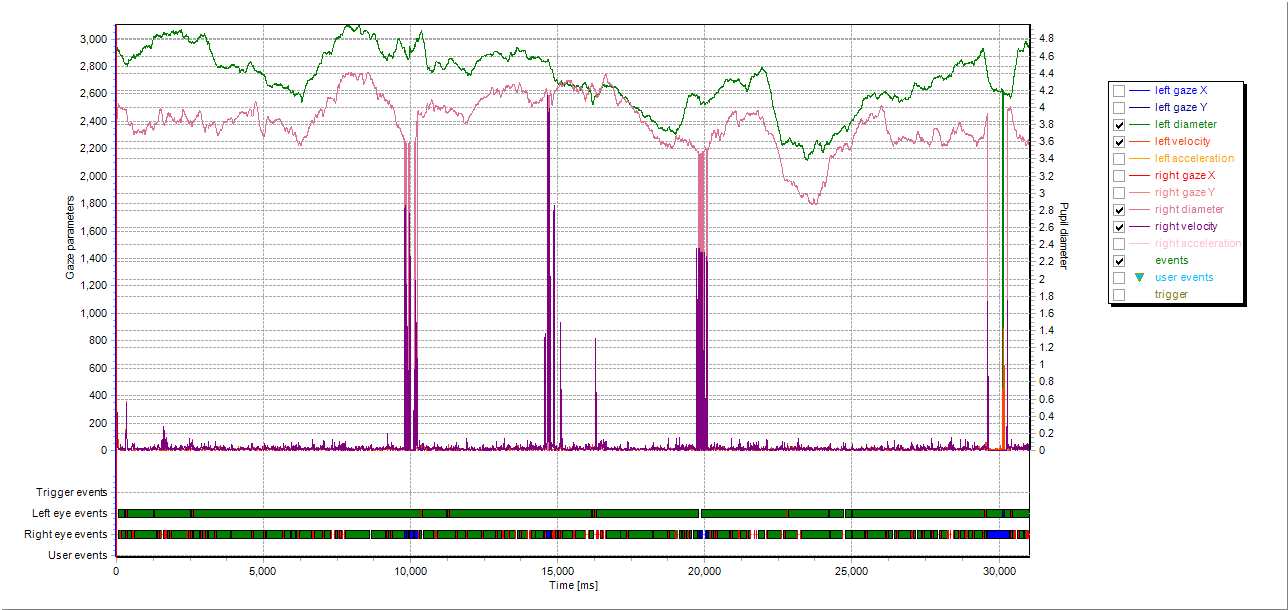
\includegraphics[width=.8\textwidth]{figures/graphs/PT_T2(triangular)_VP.png}
  \caption[PT\_T2 Eye Pupil size and velocity profile]{PT\_T2 Pupil diameter and eye velocity}
  \label{fig:PT_T2_vel}
\end{figure}

In Fig.~\ref{fig:PT_T2_vel}, it is possible to see that the during the smooth tracking the number of microsaccades appears to be lower than in the sinusoidal motion pattern. This is probably due to the fact that the triangular pattern has constant velocity, which should be easier for the oculomotor system to attune to. The three groups of large saccades are highlighted clearly by their peaks in velocity. The last peaks in velocity seem to be due more to a tracking loss.



\subsection{PT\_T3 : Step-Ramp pursuit visual stimuli}
\label{sec:PT_T3}

\begin{figure}[t]
  \centering
  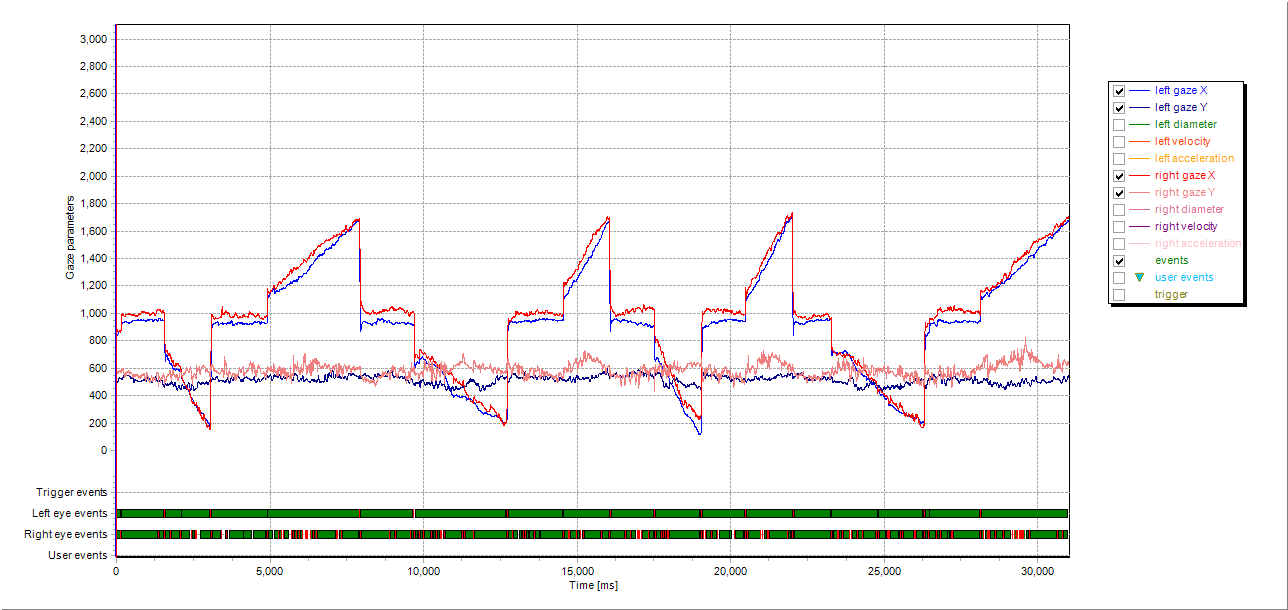
\includegraphics[width=.8\textwidth]{figures/graphs/PT_T3(stepRamp)_XY.png}
  \caption[PT\_T3 Eye positioning]{PT\_T3 Eye positioning}
  \label{fig:PT_T3_pos}
\end{figure}

\begin{figure}[t]
  \centering
  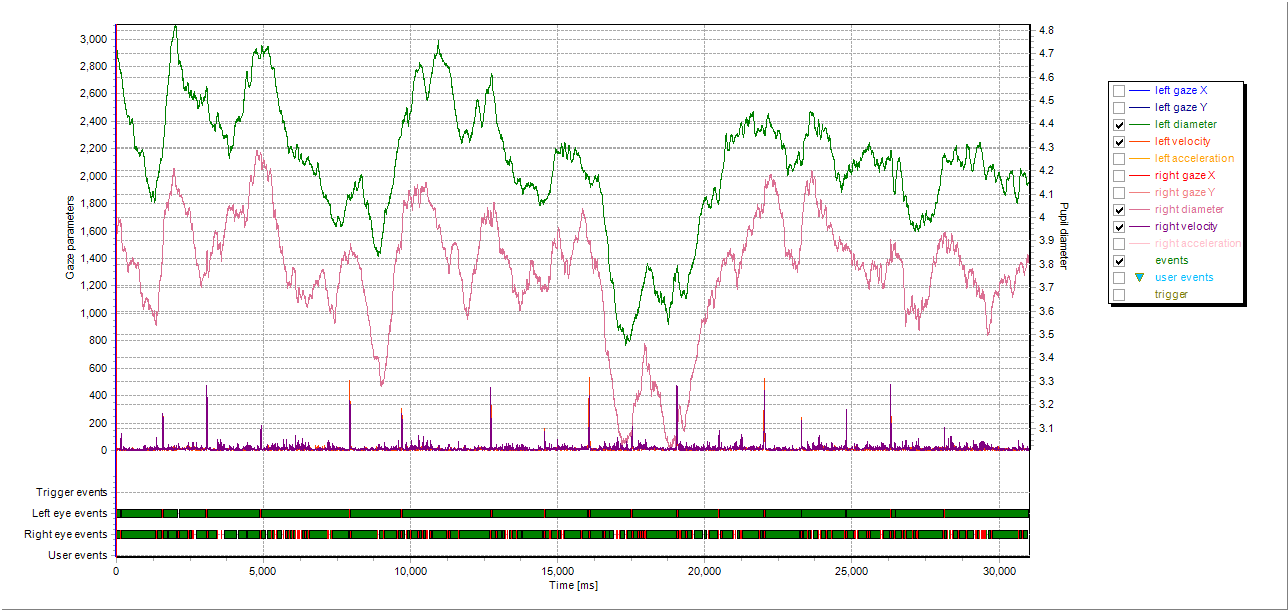
\includegraphics[width=.8\textwidth]{figures/graphs/PT_T3(stepRamp)_VP.png}
  \caption[PT\_T3 Pupil size and velocity profile]{PT\_T3 Pupil diameter and eye velocity}
  \label{fig:PT_T3_vel}
\end{figure}

In Fig.~\ref{fig:PT_T3_pos} it is fairly clear to see the step-ramp paradigm in action. The x coordinate have a baseline of 960 px (since the target was displayed at the center of the screen, at half of the size of the stimuli, therefore 1920px/2). The eyes fixates at the baseline value, then they perform a rapid saccade towards the step location of 3 deg (positive or negative, either above or below the baseline), then they follow smoothly the target towards the final location of 15 deg (above or below the baseline depending on the direction) and finally they return to the baseline position at the start of the subsequent trial. The difference in time taken for completing the ramp pursuits is due to the different velocity profiles (4 or 8 deg/s).

The y coordinates of the eye movements are always equal, since the stimuli moves only on the horizontal axis. No large saccades or blinks are visible in the recorded data.

It is important to remind that even during fixations, a number of small eye movements are performed in order to prevent visual habituation \citep[p. 3]{leigh2015neurology}, therefore a completely flat velocity profile is not expected even during fixations.

In Fig.~\ref{fig:PT_T3_vel} it is possible to see the quick burst of more or less consistent velocity performed by the eyes in order to do the necessary saccade for the step. Then the smooth pursuit during the ramp flattens the velocity profile of the eye movements in a similar way than the fixations before the step do.


\subsection{PT\_T4 : Visually guided saccades visual stimuli}
\label{sec:PT_T4}

\begin{figure}[t]
  \centering
  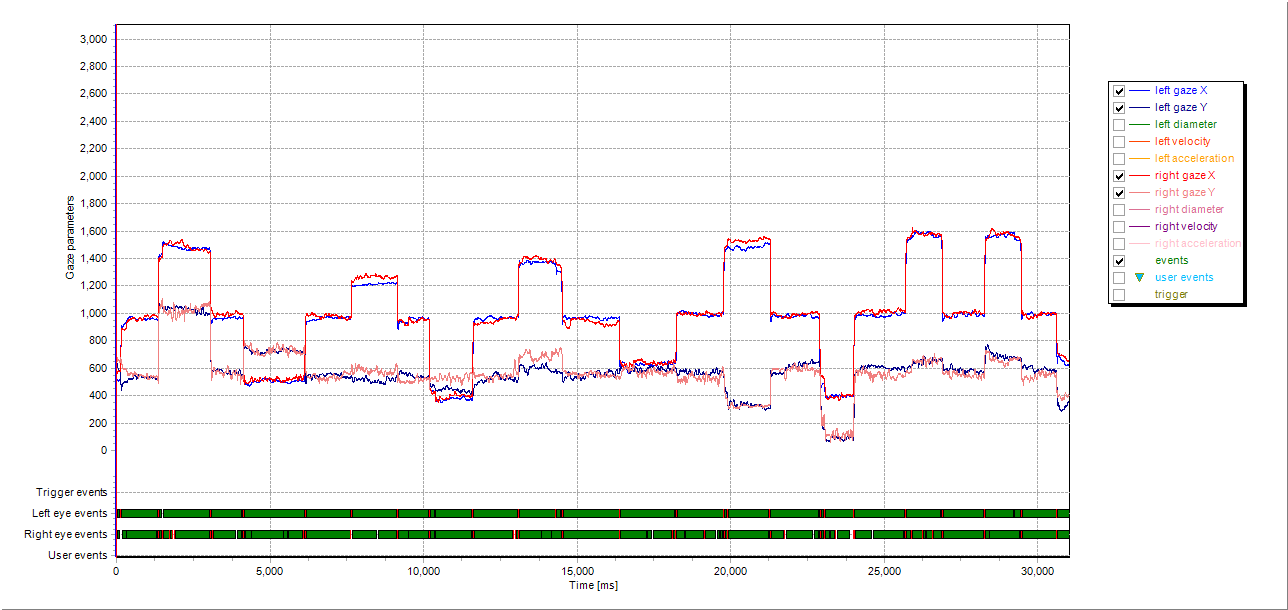
\includegraphics[width=.8\textwidth]{figures/graphs/PT_T4(saccades)_XY.png}
  \caption[PT\_T4 Eye positioning]{PT\_T4 Eye positioning}
  \label{fig:PT_T4_pos}
\end{figure}

\begin{figure}[t]
  \centering
  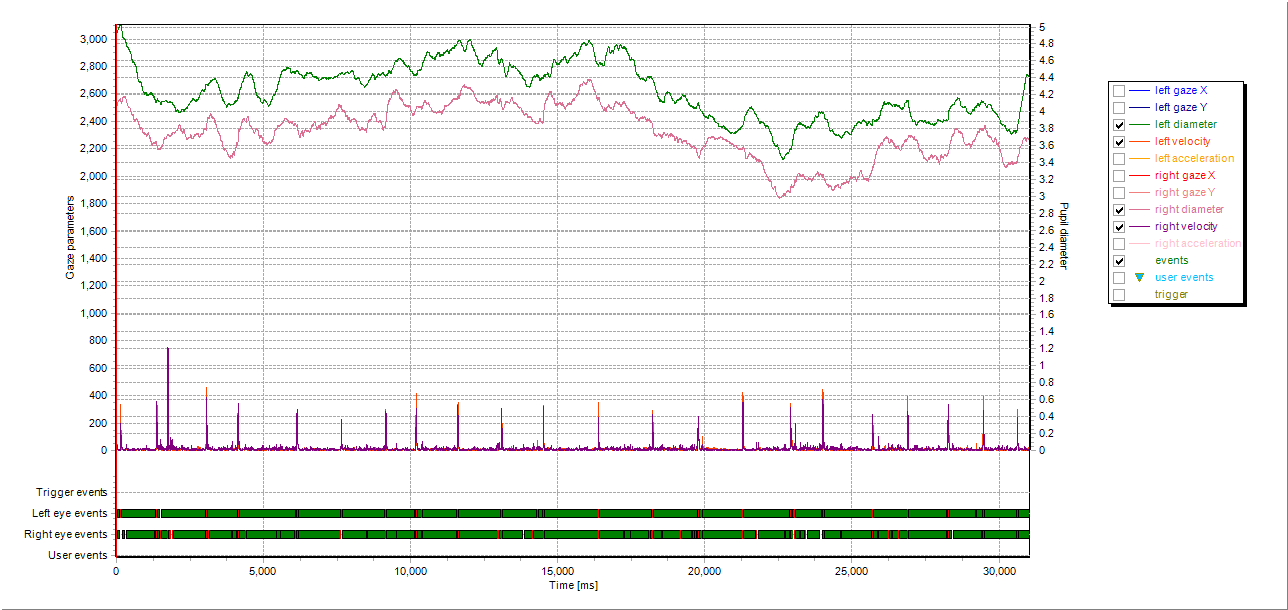
\includegraphics[width=.8\textwidth]{figures/graphs/PT_T4(saccades)_VP.png}
  \caption[PT\_T4 Pupil size and velocity profile]{PT\_T4 Pupil diameter and eye velocity}
  \label{fig:PT_T4_vel}
\end{figure}


Fig.~\ref{fig:PT_T4_pos} shows how both the x and y coordinates of the eye change abruptly when a saccade is performed in order to track the target moving freely on the screen. The baseline value for the x value is 960 px while for the y value is 540 px (half of the stimulus size, since the target is at the center). The position profile moves upward or downward from the baseline basing on the direction of the target movement. Since the target stays both in the center and in the periphery for certain amounts of time, it is possible to see the fixation stabilization in between saccades. The trial lasted 43.7 s, but the chart focuses on the first 30 s in order to provide more details.

Fig.~\ref{fig:PT_T4_vel} shows the bursts of eye velocity while performing the visually guided saccades, and the flat velocity profiles of the in-between fixations. It is interesting to notice that the first eye movement (performed between 1 and 2 seconds) has higher velocity and it is done in two saccades, therefore it was probably less precise. After that one, the other saccades are pretty similar, showing an attunement of the oculomotor system to the visual stimuli.





\section{Experimental group [P1, P2, P3]}
\label{sec:resexpgroup}

Tab.~\ref{tab:expgroupresultssummary} shows an overview of the results from the experiments with the target group (P1, P2 and P3).

\begin{table}[t]
   \centering
   \begin{tabular}{@{}c@{\hspace{.5cm}}c@{}}
       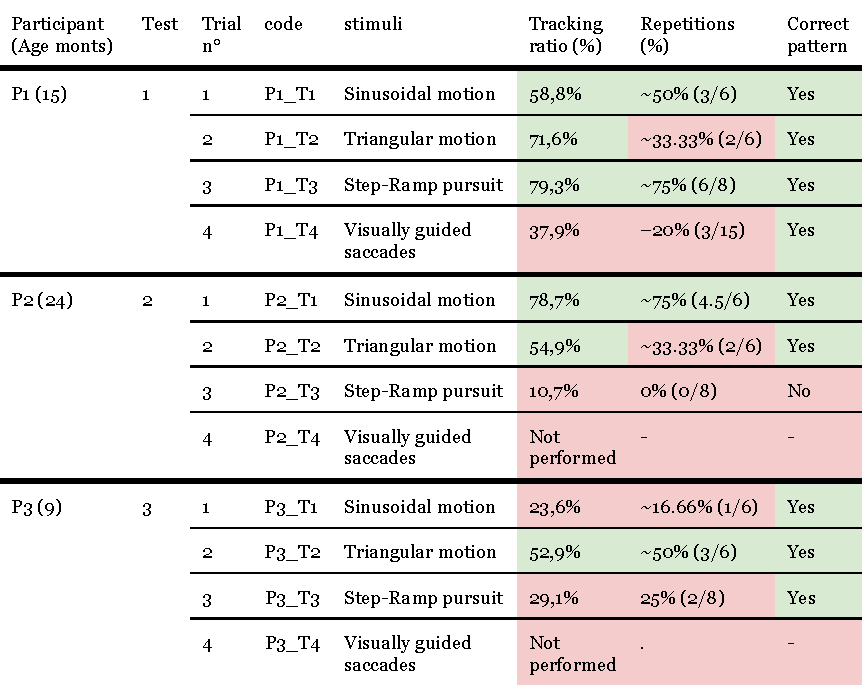
\includegraphics[page=1,width=.9\textwidth]{figures/tables/table_5.pdf}
   \end{tabular}
 \caption{P\{1,2,3\} experiments results overview.}
 \label{tab:expgroupresultssummary}
\end{table}

\pagebreak

\subsection{P\{1,2,3\}\_T1 : Sinusoidal motion visual stimuli}
\label{sec:P123_T1}

\subsubsection{P1\_T1}
\label{sec:P1_T1}

\begin{figure}[h]
  \centering
  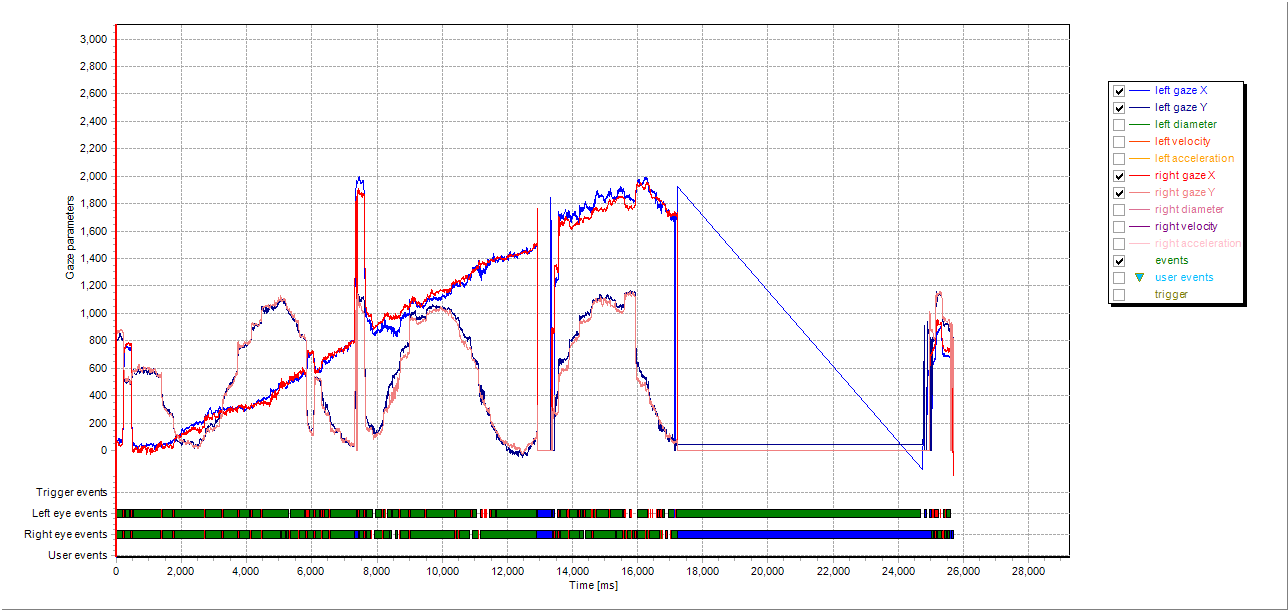
\includegraphics[width=.8\textwidth]{figures/graphs/P1_T1(sinusoid)_XY.png}
  \caption[P1\_T1 Eye positioning]{P1\_T1 Eye positioning}
  \label{fig:P1_T1_pos}
\end{figure}

The visual stimuli elicited a gaze pattern (Fig.~\ref{fig:P1_T1_pos}) pretty close to the one expected for half of the designed repetitions. Indeed, the tracking record show data until the half of the experiment, while the target was moving in one direction from left to right. The graph show how P1’s eyes did not perform a very smooth pursuit especially near to the turning points and during the third repetition. Rather, it seems that they performed more of a series of saccades and fixations, drawing a “staircase” profile.
The graph also shows the intrusion of more or less large saccades especially immediately after the target turning points, which is consistent with the pilot test data.

\begin{figure}[h]
  \centering
  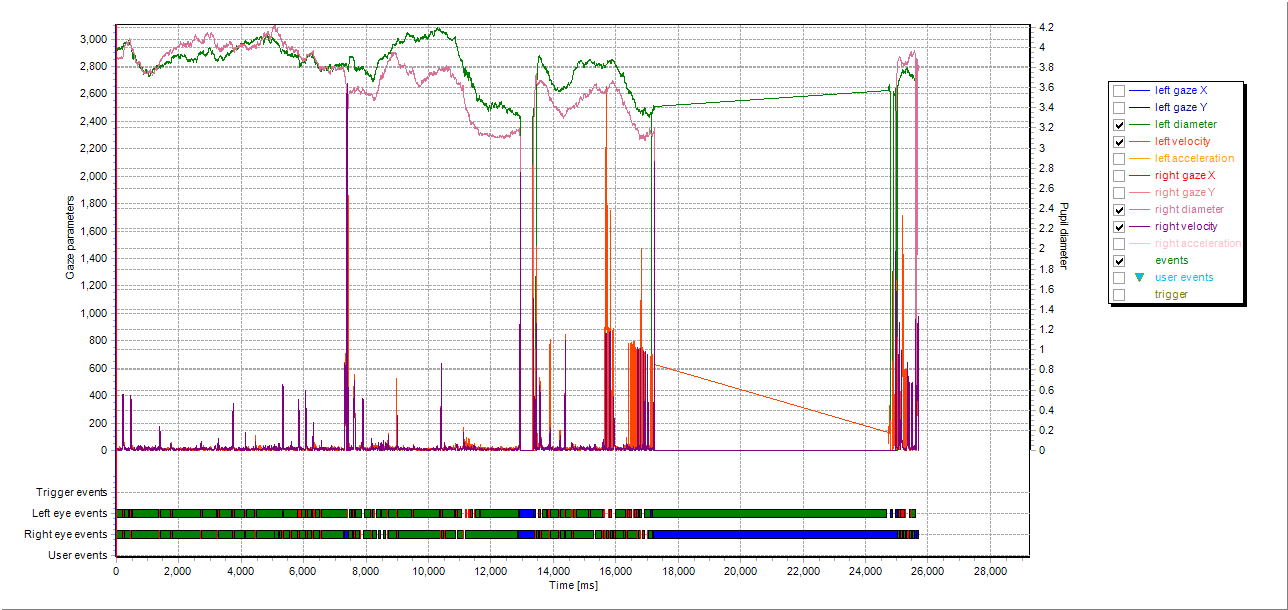
\includegraphics[width=.8\textwidth]{figures/graphs/P1_T1(sinusoid)_VP.png}
  \caption[P1\_T1 Pupil size and velocity profile]{P1\_T1 Pupil diameter and eye velocity}
  \label{fig:P1_T1_vel}
\end{figure}

Fig.~\ref{fig:P1_T1_vel} shows that during the smooth pursuit tracking in the first half of the stimuli presentation, P1 performed a series of small corrective saccades with small peaks of velocity, and also three large saccades with bursts of high peaks of velocity after the target turning points, where the eye velocity profile flattens the most since the target velocity is at minimum.



\subsubsection{P2\_T1}
\label{sec:P2_T1}

\begin{figure}[h]
  \centering
  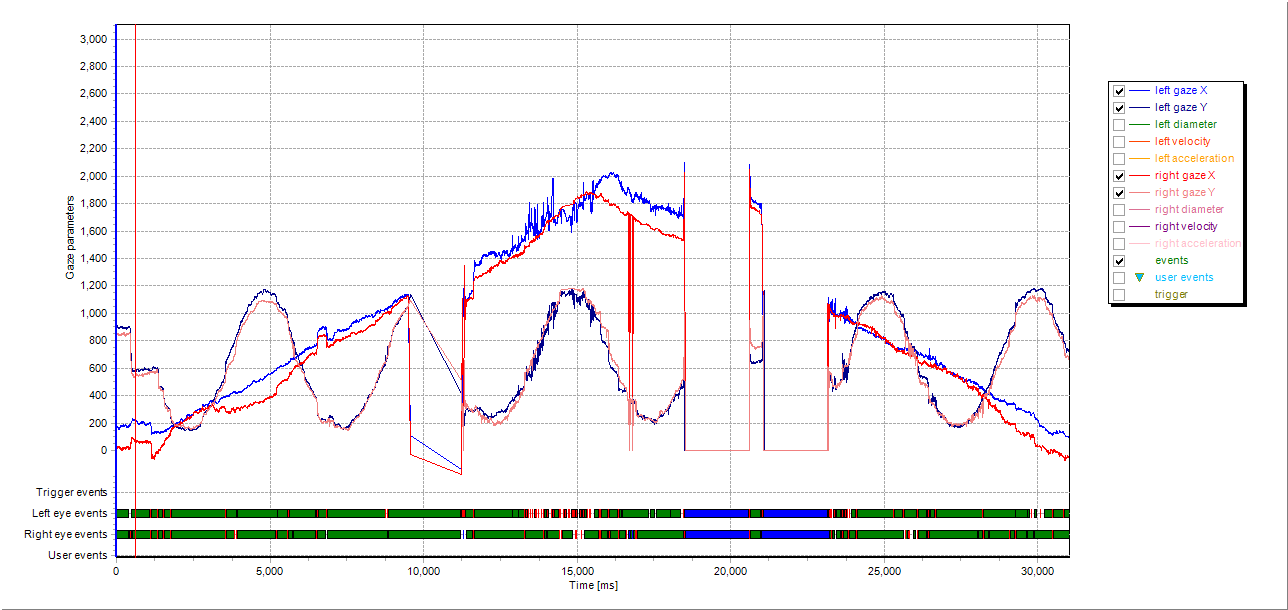
\includegraphics[width=.8\textwidth]{figures/graphs/P2_T1(sinusoid)_XY.png}
  \caption[P2\_T1 Eye positioning]{P2\_T1 Eye positioning}
  \label{fig:P2_T1_pos}
\end{figure}

Fig.~\ref{fig:P2_T1_pos} shows that P2 tracked the sinusoidal moving target smoothly with noticeable accuracy throughout all the stimuli presentation. The eye tracker lost data on one full repetition and a half one, probably because the child moved a bit far away from the eye tracker or something caught her attention elsewhere. However, she returned to track the target again accurately. Two saccades, a small one and a large one, are visible before the target turning points, when the target starts decelerating noticeably.

\begin{figure}[h]
  \centering
  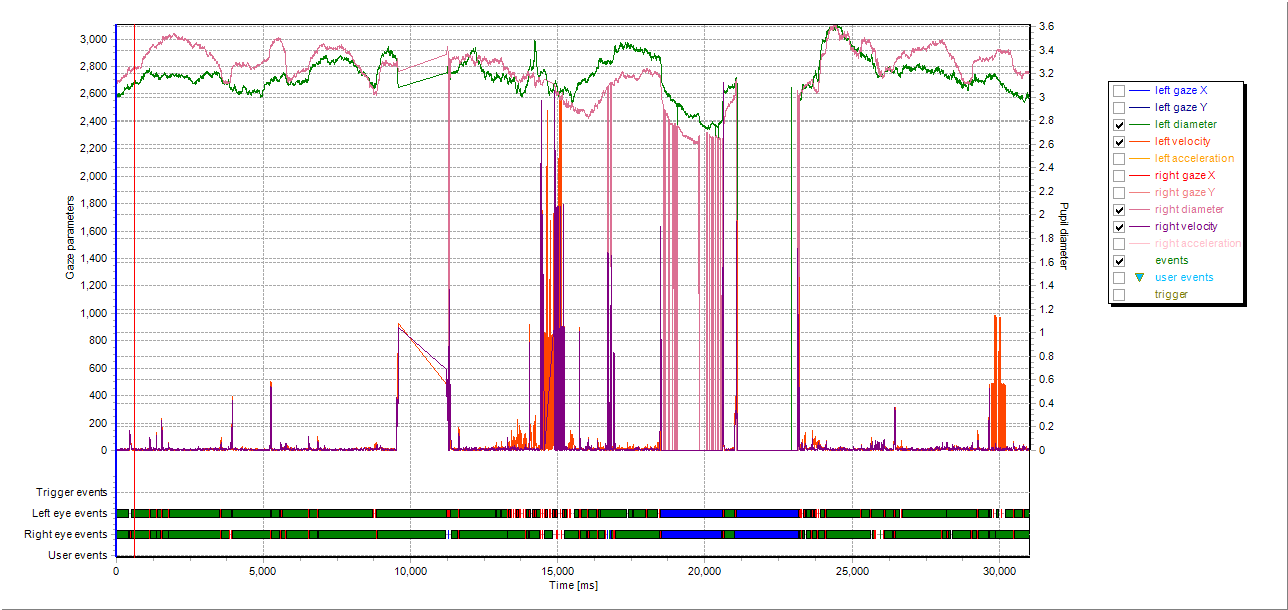
\includegraphics[width=.8\textwidth]{figures/graphs/P2_T1(sinusoid)_VP.png}
  \caption[P2\_T1 Pupil size and velocity profile]{P2\_T1 Pupil diameter and eye velocity}
  \label{fig:P2_T1_vel}
\end{figure}

Fig.~\ref{fig:P2_T1_vel} show how during smooth tracking the velocity profile of P2 eyes is near to be flat, meaning that even though the eyes were moving constantly, P2 made no saccades or abrupt eye movements. Bursts of high peaks of eye velocity are found during larger saccades intrusions.



\subsubsection{P3\_T1}
\label{sec:P3_T1}

\begin{figure}[t]
  \centering
  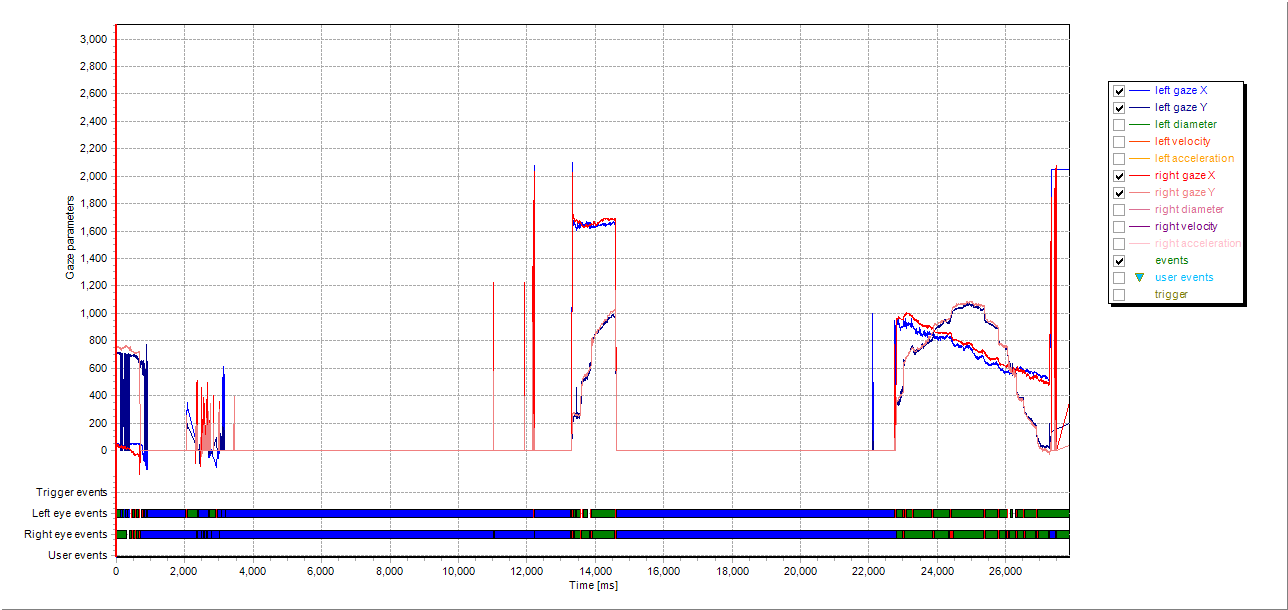
\includegraphics[width=.8\textwidth]{figures/graphs/P3_T1(sinusoid)_XY.png}
  \caption[P3\_T1 Eye positioning]{P3\_T1 Eye positioning}
  \label{fig:P3_T1_pos}
\end{figure}

As Fig.~\ref{fig:P3_T1_pos} shows, the quantity of collected data from P3 in the first trial is rather low (tracking ratio 23,6\%). This is probably due to the fact that the child might become comfortable to sit in a position too far away from the display monitor. Or it can be due to the fact that the child seemed very curious towards the researchers and was more keen on observing them than the display monitor. These events are expected to happen while testing with such a small baby. Therefore, it is not possible to state that the recorded data can be useful for an in-deep analysis. However, in the only full repetition completely recorded as well as in the first section of another one, it is possible to see that the stimuli elicited the expected sinusoidal gaze pattern. Moreover, the smooth tracking shows qualitatively the same staircase profile of P1.

\begin{figure}[t]
  \centering
  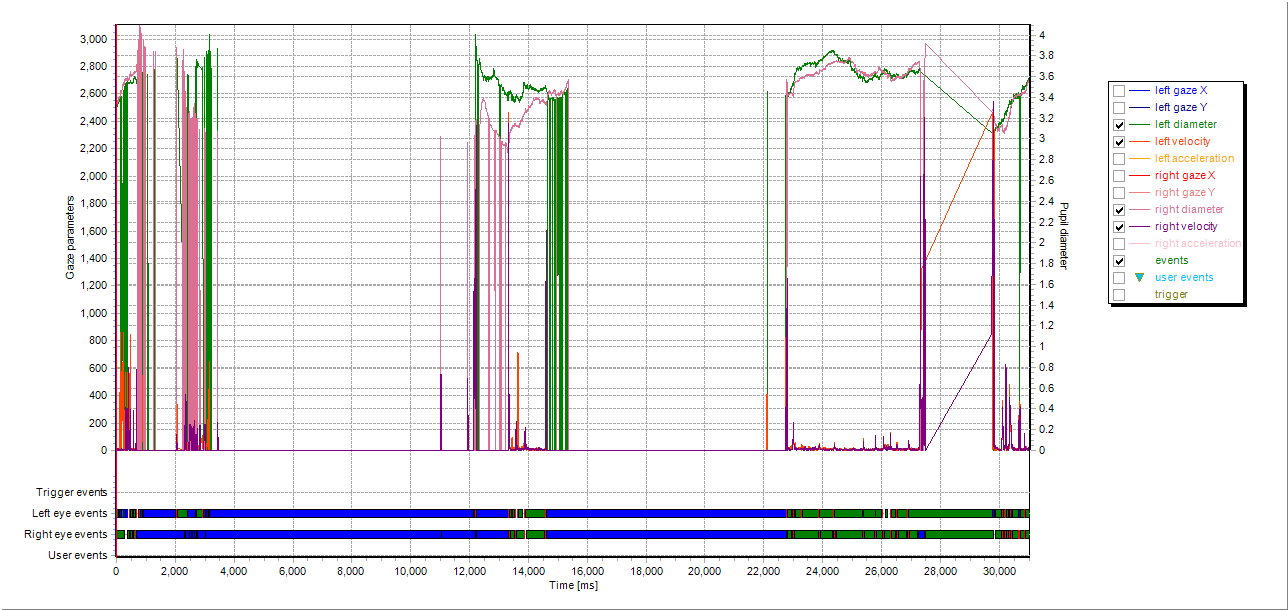
\includegraphics[width=.8\textwidth]{figures/graphs/P3_T1(sinusoid)_VP.png}
  \caption[P3\_T1 Pupil size and velocity profile]{P3\_T1 Pupil diameter and eye velocity}
  \label{fig:P3_T1_vel}
\end{figure}

In the only two clear record sets available (Fig.~\ref{fig:P3_T1_vel}), it is possible to see that a number of small saccades with low peaks of velocity are performed during the smooth tracking with a more flat velocity profile. The pattern is visually pretty stable, suggesting a good control over the eye movements performed, regardless their performance.



\subsection{P\{1,2,3\}\_T2 : Triangular motion visual stimul}
\label{sec:P123_T2}

\subsubsection{P1\_T2}
\label{sec:P1_T2}

\begin{figure}[t]
  \centering
  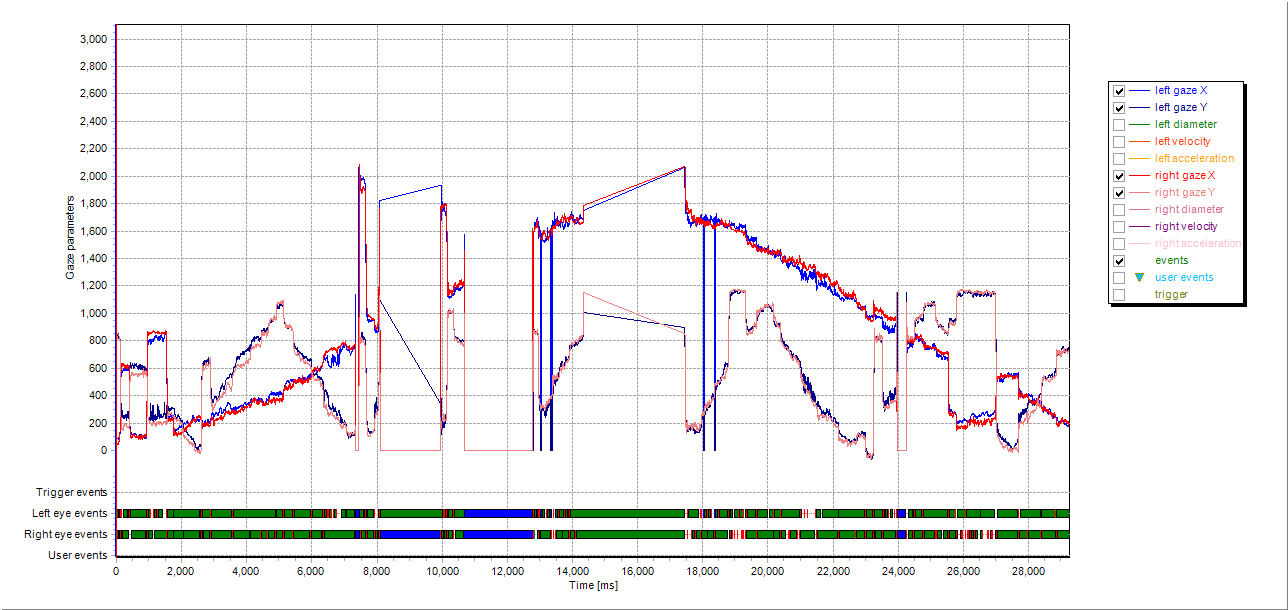
\includegraphics[width=.8\textwidth]{figures/graphs/P1_T2(triangular)_XY.png}
  \caption[P1\_T2 Eye positioning]{P1\_T2 Eye positioning}
  \label{fig:P1_T2_pos}
\end{figure}

\begin{figure}[t]
  \centering
  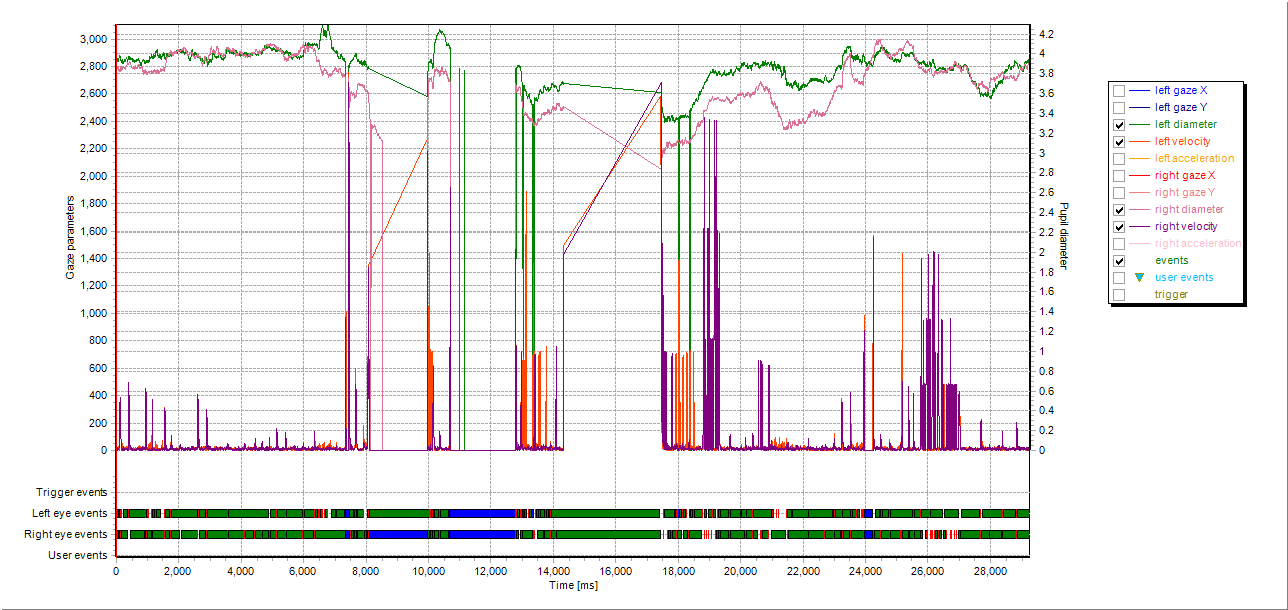
\includegraphics[width=.8\textwidth]{figures/graphs/P1_T2(triangular)_VP.png}
  \caption[P1\_T2 Pupil size and velocity profile]{P1\_T2 Pupil diameter and eye velocity}
  \label{fig:P1_T2_vel}
\end{figure}

In Fig.~\ref{fig:P1_T2_pos} it is possible to spot the triangular motion pattern, however large and small saccades are present throughout the whole record. A couple of full repetitions are clean from saccadic intrusions. The smooth tracking shows a staircase profile, like for the sinusoidal motion stimuli, but it seems less abrupt in this stimuli. This could be due to the fact that the velocity profile of the triangular motion remains constant, resulting in being more predictable and easier to track smoothly for the child.

Fig.~\ref{fig:P1_T2_vel} shows the presence of small saccades intruding the smooth pursuit even in the two cleaner repetitions.


\subsubsection{P2\_T2}
\label{sec:P2_T2}

\begin{figure}[t]
  \centering
  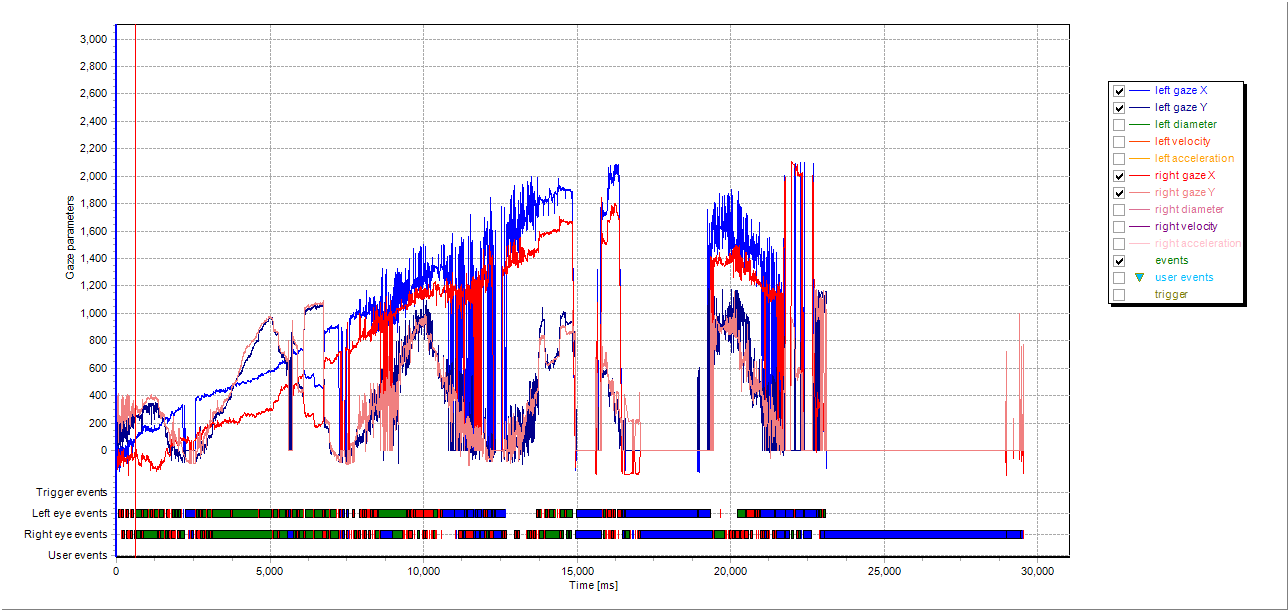
\includegraphics[width=.8\textwidth]{figures/graphs/P2_T2(triangular)_XY.png}
  \caption[P1\_T2 Eye positioning]{P2\_T2 Eye positioning}
  \label{fig:P2_T2_pos}
\end{figure}

\begin{figure}[t]
  \centering
  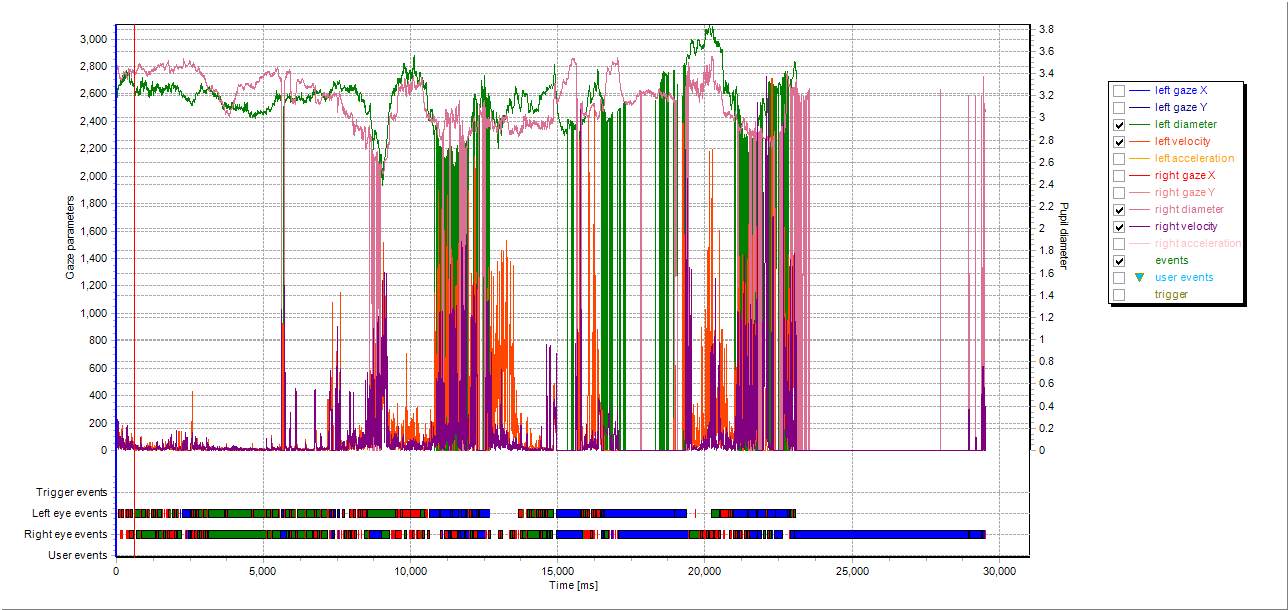
\includegraphics[width=.8\textwidth]{figures/graphs/P2_T2(triangular)_VP.png}
  \caption[P2\_T2 Pupil size and velocity profile]{P2\_T2 Pupil diameter and eye velocity}
  \label{fig:P2_T2_vel}
\end{figure}

The graph for the triangular pursuit of P2 (Fig.~\ref{fig:P2_T2_pos})  is particularly rich of artifacts, which are particularly irregular and therefore probably due more to movements of the head or the whole body of the child rather than being caused by only by eye movements. Indeed, the dense repetition of quick eye movements, starting from the second repetition of the triangular wave, can be better explained by the child trying to track the object while keeping moving on the lap of her mother. In the record of the first clean repetition of the stimuli it is possible to see that the smooth tracking is pretty precise for the y coordinate of the eye, while the left eye leads the right one in terms of x coordinate. This might be due to the fact that the child’s head was a bit tilted or the calibration was not precise due to the movements of the child. Overall, the record does not seem to provide many reliable measurements for smooth pursuit eye movements. It is possible that the stimuli was not different enough from the previous one in order to be interesting enough for the child, or she felt uncomfortable to sit still in position at the moment of this trial.

Fig.~\ref{fig:P2_T2_vel} shows how only the first repetition of the stimuli shows eye tracking with a velocity profile clean an flat enough to be considered smooth pursuit. The rest of the record is too noisy to be considered.




\subsubsection{P3\_T2}
\label{sec:P3_T2}

\begin{figure}[t]
  \centering
  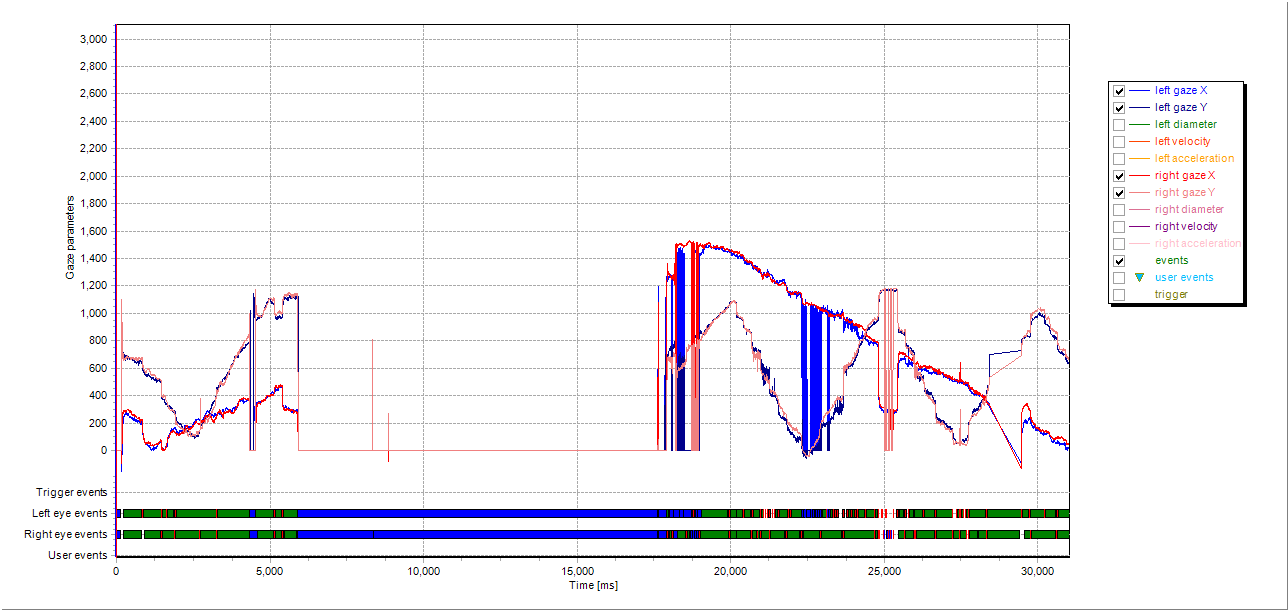
\includegraphics[width=.8\textwidth]{figures/graphs/P3_T2(triangular)_XY.png}
  \caption[P3\_T2 Eye positioning]{P3\_T2 Eye positioning}
  \label{fig:P3_T2_pos}
\end{figure}

\begin{figure}[t]
  \centering
  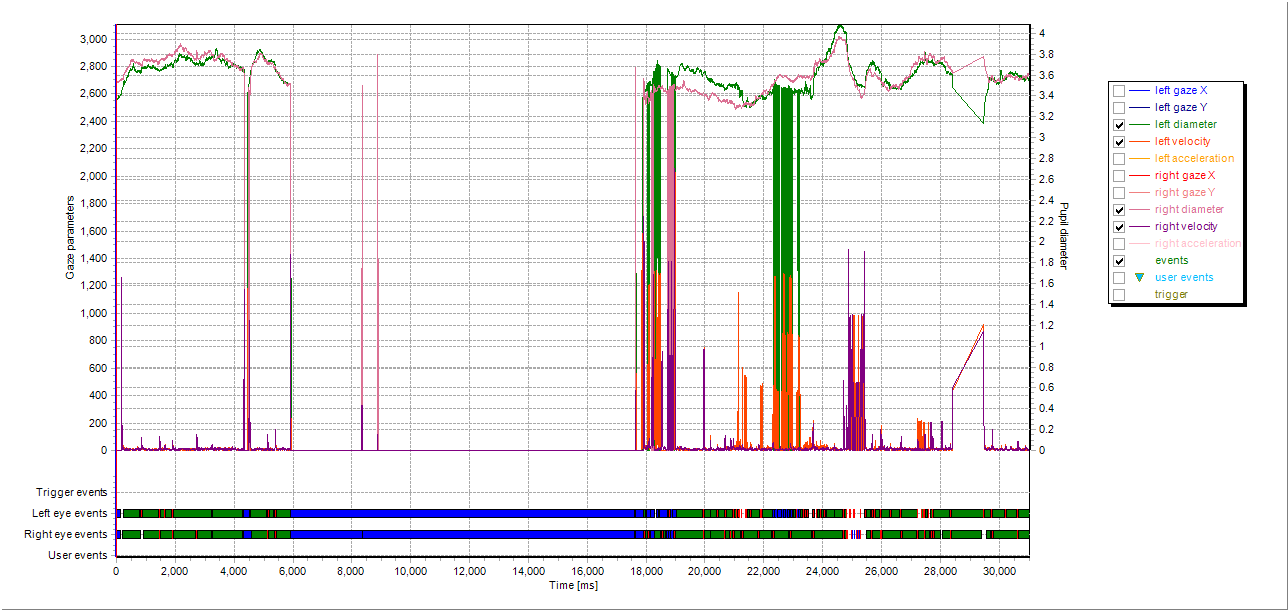
\includegraphics[width=.8\textwidth]{figures/graphs/P3_T2(triangular)_VP.png}
  \caption[P3\_T2 Pupil size and velocity profile]{P3\_T2 Pupil diameter and eye velocity}
  \label{fig:P3_T2_vel}
\end{figure}

The tracking record of P3 (Fig.~\ref{fig:P3_T2_pos}) is pretty accurate, she followed the stimuli mainly during the second part of the presentation. Large saccades are visible at the target turning points, as predictable, both on the horizontal and vertical axes. A staircase profile for the smooth tracking is present also in this stimuli. Overall the stimuli seemed to work  well in eliciting the expected gaze pattern. The central part of the record is missing, probably because the child looked away for some time.

Fig.~\ref{fig:P3_T2_vel} shows how in the first repetition of the stimuli few saccades with small peaks in velocity disrupted an otherwise pretty flat eye velocity profile, suggesting smooth tracking. On the other hand, In the second part of the stimuli more and larger saccades intruded the smooth tracking.


\subsection{P\{1,2,3\}\_T3 : Step-Ramp pursuit visual stimuli}
\label{sec:P123_T3}

\subsubsection{P1\_T3}
\label{sec:P1_T3}

\begin{figure}[t]
  \centering
  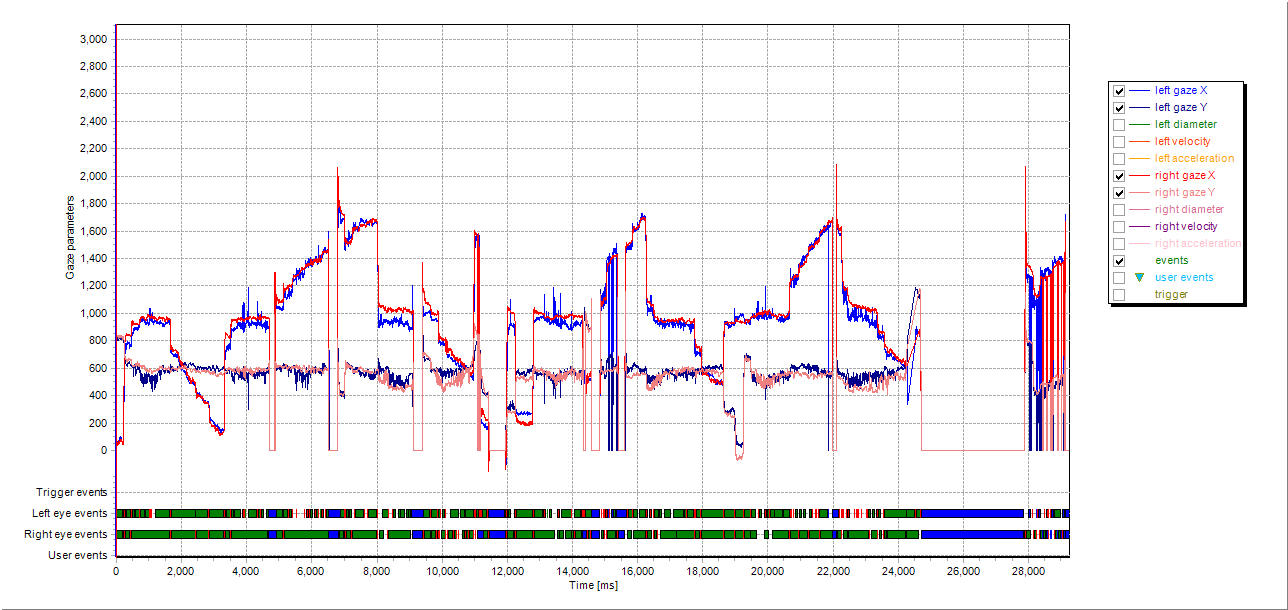
\includegraphics[width=.8\textwidth]{figures/graphs/P1_T3(stepRamp)_XY.png}
  \caption[P1\_T3 Eye positioning]{P1\_T3 Eye positioning}
  \label{fig:P1_T3_pos}
\end{figure}

\begin{figure}[t]
  \centering
  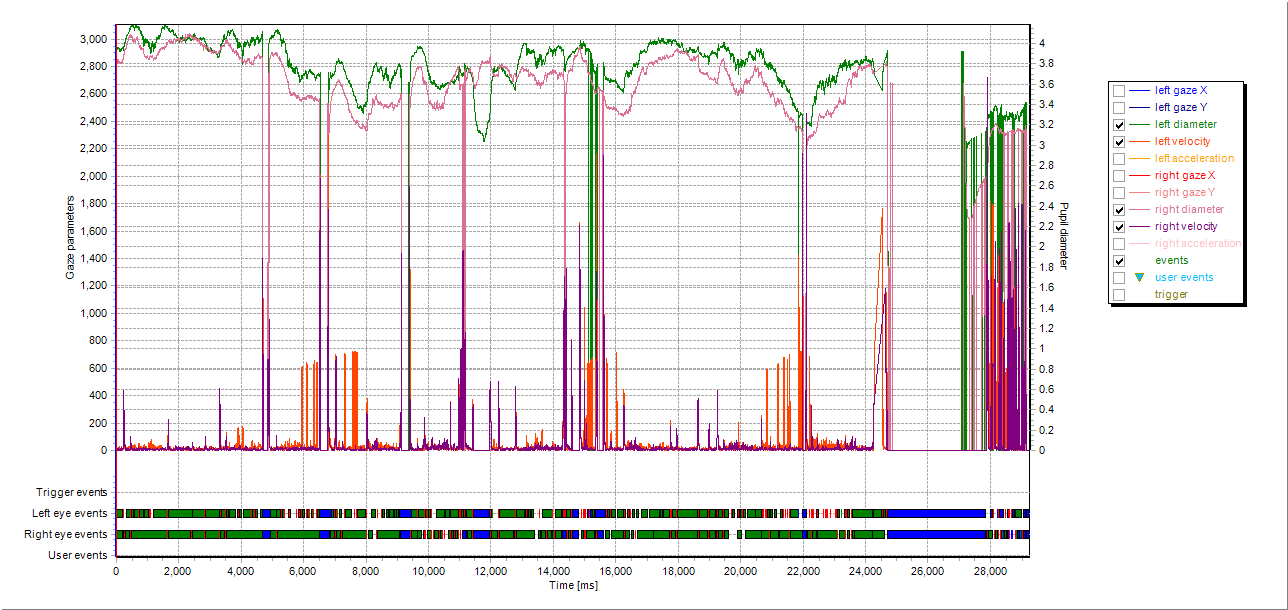
\includegraphics[width=.8\textwidth]{figures/graphs/P1_T3(stepRamp)_VP.png}
  \caption[P1\_T3 Pupil size and velocity profile]{P1\_T3 Pupil diameter and eye velocity}
  \label{fig:P1_T3_vel}
\end{figure}

Fig.~\ref{fig:P1_T3_pos} shows pretty clearly that the stimuli elicited the expected eye movements. All the phases of the paradigm are easily detectable (initial \textit{fixation}, \textit{step} saccade, smooth pursuit \textit{ramp}). A number of large saccade is visible, happening in particular moments (e.g. during the step, or when the target returns to the central point after the end of a repetition). Some of them might be also blinks, since they happen in the middle of pursuit tracking, where no competing stimuli or abrupt target movements are shown. The tracking appears accurate, and the staircase pattern is visible only in some parts of the chart.



Fig.~\ref{fig:P1_T3_vel} shows the presence of a series of saccades with consistent velocity, around 400 deg/s, which happen at during the step phase. The other larger saccades with higher peaks of velocity can be considered as intrusive of either fixations or smooth pursuit. The velocity profile, when not disrupted by saccades, appears fairly flat, indicating somewhat stable fixations and smooth pursuits. 



\subsubsection{P2\_T3}
\label{sec:P2_T3}

The eye tracking data of P2 during the step-ramp visual stimuli are insufficient for being analyzed (Fig.~\ref{fig:P2_T3_pos}). Indeed, at this point of the experiment P2 seemed tired of watching at the display monitor. Probably the experiment was lasting for too long, and she lost interest. Indeed, the researchers and P2’s mother decided to stop the experiment and leave the child to go outside to play with her friends. P2 did not perform further trials.

\begin{figure}[h]
  \centering
  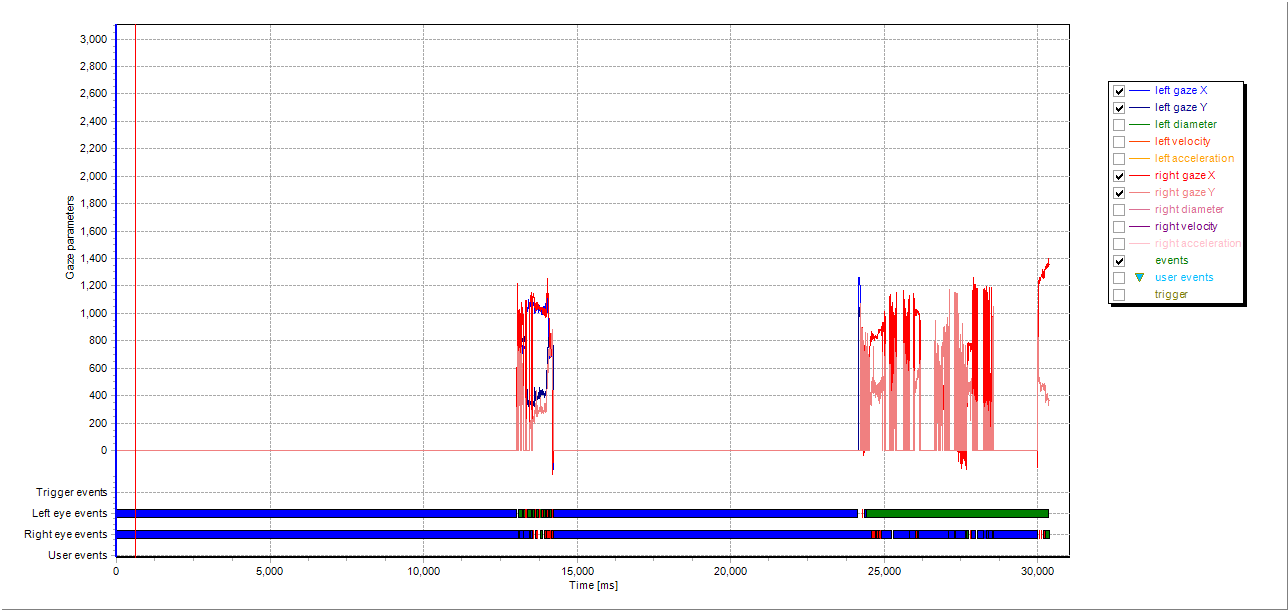
\includegraphics[width=.8\textwidth]{figures/graphs/P2_T3(stepRamp)_XY.png}
  \caption[P2\_T3 Eye positioning]{P2\_T3 Eye positioning}
  \label{fig:P2_T3_pos}
\end{figure}



\subsubsection{P3\_T3}
\label{sec:P3_T3}

The record for the step-ramp stimuli of P3 stops after the second repetition. After that moment, P3 started interacting with her sister and her mother. She was probably a bit tired to look at the display monitor too. However, the recorded data show interesting patterns.

\begin{figure}[h]
  \centering
  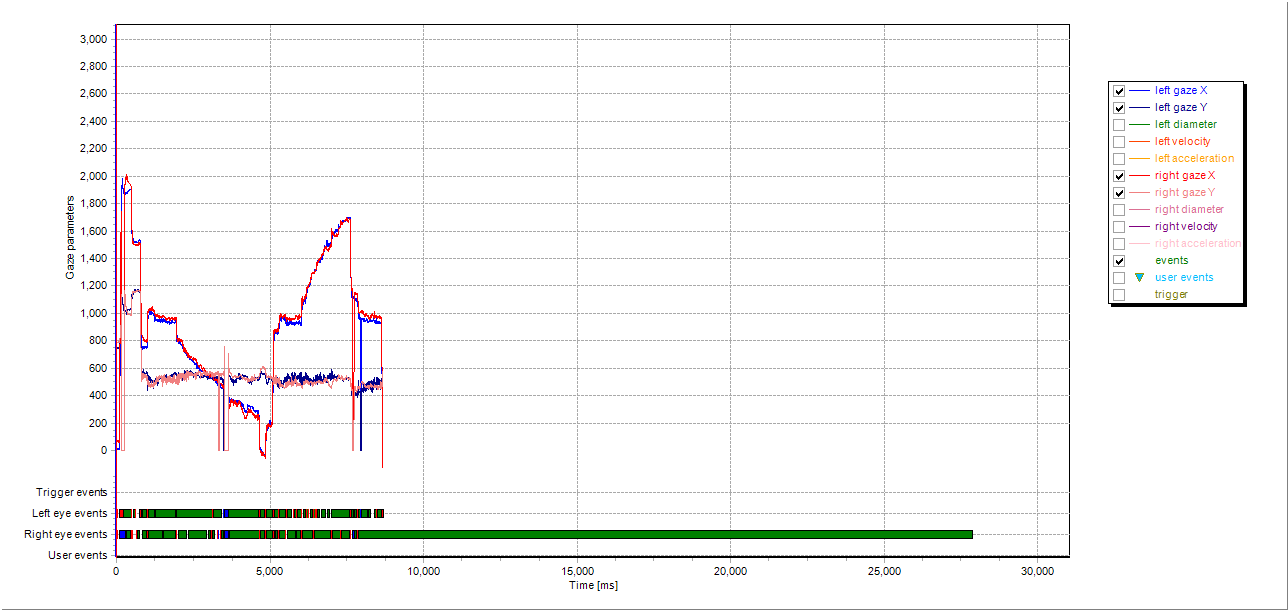
\includegraphics[width=.8\textwidth]{figures/graphs/P3_T3(stepRamp)_XY.png}
  \caption[P3\_T3 Eye positioning]{P3\_T3 Eye positioning}
  \label{fig:P3_T3_pos}
\end{figure}

The two repetitions performed by P3 (Fig.~\ref{fig:P3_T3_pos})  show a gaze pattern which is pretty close to the expected one, with apparent good accuracy. An artifact is present during the ramp of the first repetition, and it could be a blink. While a large saccade performed after the ramp of the second repetition seems more an overshooting of the target.

\begin{figure}[h]
  \centering
  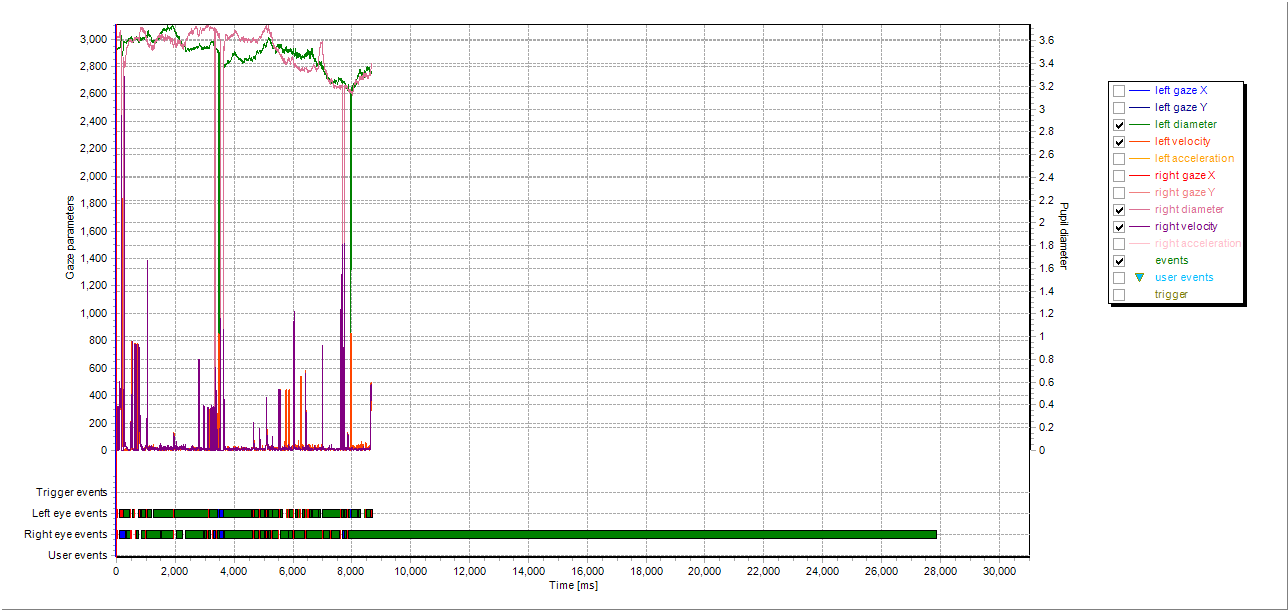
\includegraphics[width=.8\textwidth]{figures/graphs/P3_T3(stepRamp)_VP.png}
  \caption[P3\_T3 Pupil size and velocity profile]{P3\_T3 Pupil diameter and eye velocity}
  \label{fig:P3_T3_vel}
\end{figure}

Fig.~\ref{fig:P3_T3_vel} reveals how the velocity profile of the smooth pursuit ramp of the first repetition is overall flat, if not considering the artifact in between the pursuit, indicating smooth tracking. On the other hand, the series of peaks of eye velocity during the second ramp suggest more of a staircase pattern, with saccades and fixations in sequence rather a single smooth pursuit.

\subsection{P\{1,2,3\}\_T4 : Visually guided saccades visual stimuli}
\label{sec:P123_T4}


\subsubsection{P1\_T4}
\label{sec:P1_T4}

\begin{figure}[t]
  \centering
  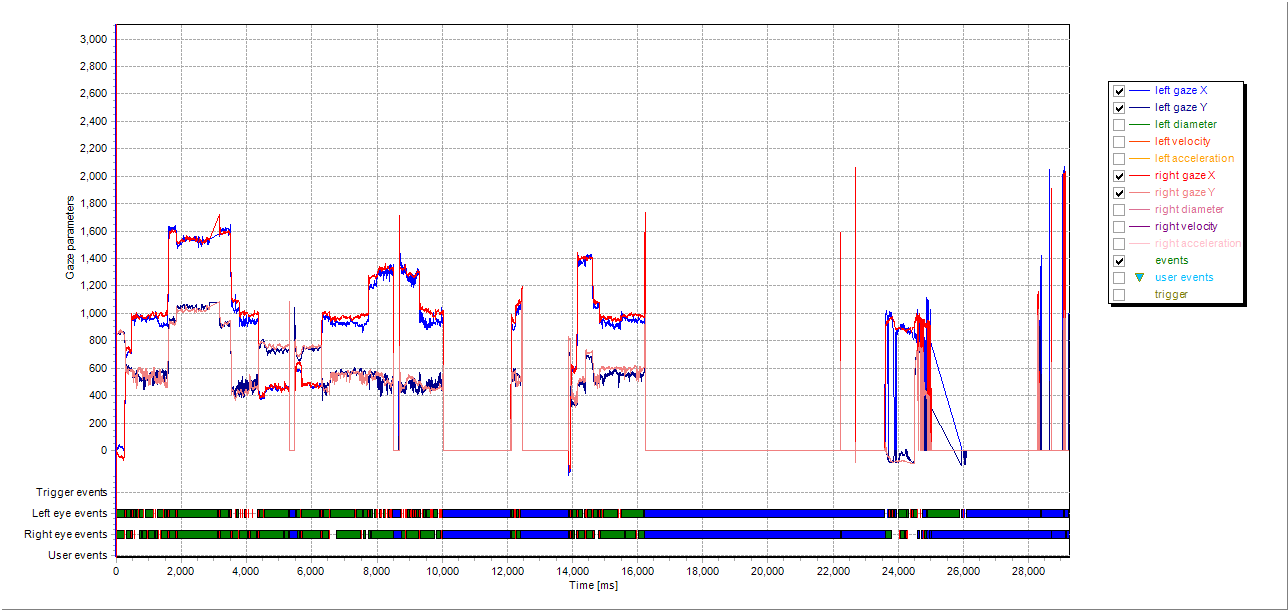
\includegraphics[width=.8\textwidth]{figures/graphs/P1_T4(saccades)_XY.png}
  \caption[P1\_T4 Eye positioning]{P1\_T4 Eye positioning}
  \label{fig:P1_T4_pos}
\end{figure}

\begin{figure}[t]
  \centering
  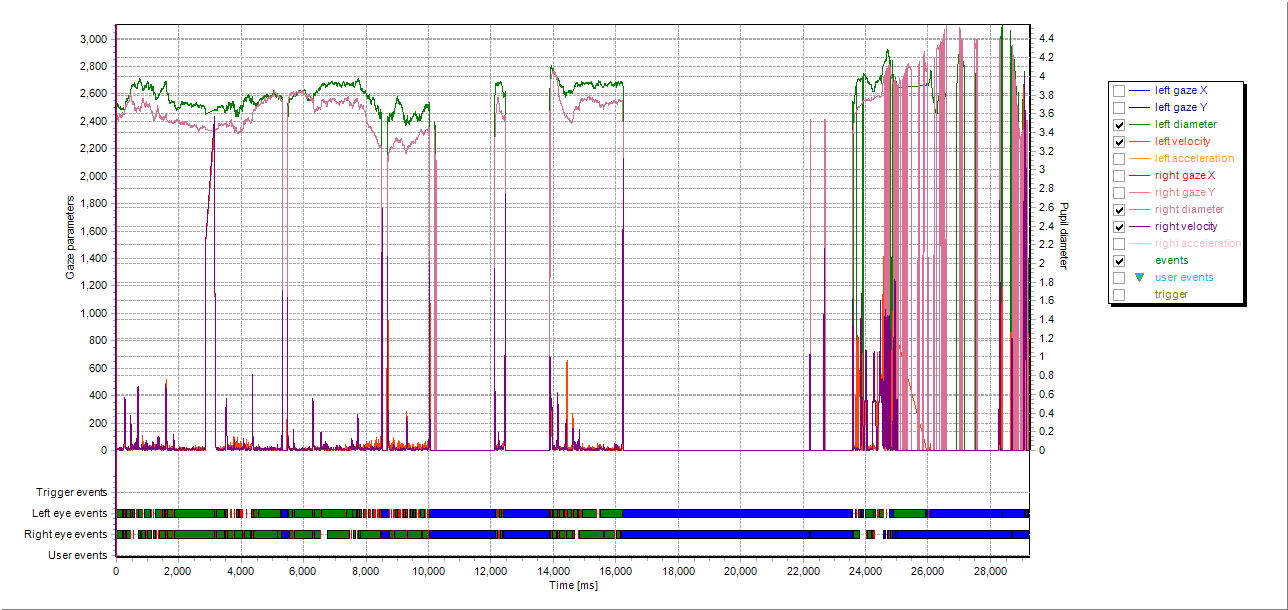
\includegraphics[width=.8\textwidth]{figures/graphs/P1_T4(saccades)_VP.png}
  \caption[P1\_T4 Pupil size and velocity profile]{P1\_T4 Pupil diameter and eye velocity}
  \label{fig:P1_T4_vel}
\end{figure}

Fig.~\ref{fig:P1_T4_pos} show that the stimuli elicited the expected gaze pattern. A series of fixation on different points in the space is disrupted by quick eye movements, which are saccades. The fixation stabilization seems less precise from the pilot test reference dataset, and this could be due to small movement of the baby during the trial, or that the gaze stabilization improves further later in the children’s development. Some large artifacts are visible during fixations, and they probably are blinks, since they do not happen when the target moves from the center to the periphery or back.
The trial should have lasted for 43.7 s, but it has been stopped at 34.61 s since the child was evidently tired and not paying attention to the stimuli anymore. The chart shows the first 30 s, however no more evident gaze patterns are shown after 16 s.

Fig.~\ref{fig:P1_T4_vel} shows a series of consistent saccades, varying in peaks of velocity according to the amplitude of the saccade required, and in-between flatter velocity profiles of fixations, which however show constant low velocity small movements. Higher peaks in eye velocity are related to artifacts in the record, probably blinks. After 16 s the record seems to be too unreliable for being analyzed.

P2 and P3 did not perform Trial 4 (the visually guided saccades stimuli), and also P1 attended it for around one third of the time according to the tracking ratio. It seems that the experiment lasted for too long at this point, and the children’s attention faded in between the third stimulus and the third interstimulus material presentations. This made difficult to record data on Trial 4.

\subsection{Experiment notes}
\label{sec:expnotes}

Along with the eye tracker recordings, the researcher took some written notes during the experiments.

After finding a suitable spot in the home environment, P1’s calibration routines worked surprisingly good. They were fast and accurate, and the child did not need particular prompting for following the target with her gaze.
P2, during the experiment, was not particularly attracted by the first calibration procedure, which prevented to move on to the subsequent stimuli. Her mother then asked the researchers if she could help in directing P2’s attention toward the screen. The researchers welcomed the proposal, and the mother started to tell the children sentences like “what there is on the screen?” or “look at the screen”, and she pointed with her finger to the target. The mother performed this active reinforcement throughout all the experiment, and allowed to recover the child’s focus. The reinforcement was particularly useful during the calibration phases, which became shorter due to the child’s precise gaze directioning.

When a stimuli disappeared, the child often said “det er borte!” (“it disappeared!”, in English). She seemed surprised from the abrupt change between stimuli and interstimulus materials, especially in terms of the target picture. It is possible that she was expecting to see the same target performing different actions throughout the experiment stimuli. However, not meeting the child expectations fully can be a good way to keep his/her interest.\\
P2’s mother described that the child usually does not watch much television in general.

P3, the youngest participant, seemed particularly pleased with both the stimuli and the interstimulus materials. She giggled briefly when she saw the stimuli for the first time. She seemed very curious about the researchers’ presence, which made her turn frequently towards them and not following the stimuli materials on the screen. However, this reaction was expected. She was also younger than the target group, therefore the whole procedure was not completely tailored around children of her age group.